\tikzset{every picture/.style={line width=0.75pt}} %set default line width to 0.75pt        

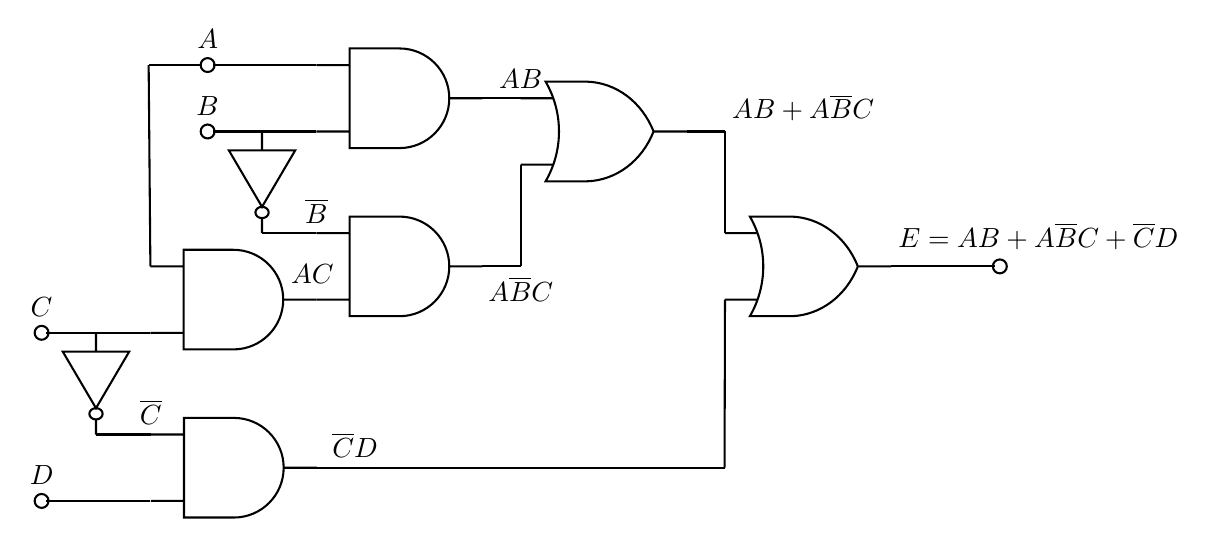
\begin{tikzpicture}[x=0.75pt,y=0.75pt,yscale=-1,xscale=1]
%uncomment if require: \path (0,393); %set diagram left start at 0, and has height of 393

%Straight Lines [id:da23815456210484298] 
\draw    (189.71,157) -- (139.64,157) ;
\draw [shift={(137.29,157)}, rotate = 180] [color={rgb, 255:red, 0; green, 0; blue, 0 }  ][line width=0.75]      (0, 0) circle [x radius= 3.35, y radius= 3.35]   ;
%Straight Lines [id:da04610179645106571] 
\draw    (189.71,189) -- (139.64,189) ;
\draw [shift={(137.29,189)}, rotate = 180] [color={rgb, 255:red, 0; green, 0; blue, 0 }  ][line width=0.75]      (0, 0) circle [x radius= 3.35, y radius= 3.35]   ;
%Straight Lines [id:da7638407091081825] 
\draw    (109.71,286) -- (59.64,286) ;
\draw [shift={(57.29,286)}, rotate = 180] [color={rgb, 255:red, 0; green, 0; blue, 0 }  ][line width=0.75]      (0, 0) circle [x radius= 3.35, y radius= 3.35]   ;
%Shape: And Gate [id:dp1564557077664277] 
\draw   (205.71,149) -- (229.71,149) .. controls (242.96,149) and (253.71,159.75) .. (253.71,173) .. controls (253.71,186.25) and (242.96,197) .. (229.71,197) -- (205.71,197) -- (205.71,149) -- cycle (189.71,157) -- (205.71,157) (189.71,189) -- (205.71,189) (253.71,173) -- (269.71,173) ;
%Straight Lines [id:da4661863224212748] 
\draw    (288.13,173) -- (269.71,173) ;
%Straight Lines [id:da3326289809840617] 
\draw    (109.71,367) -- (59.64,367) ;
\draw [shift={(57.29,367)}, rotate = 180] [color={rgb, 255:red, 0; green, 0; blue, 0 }  ][line width=0.75]      (0, 0) circle [x radius= 3.35, y radius= 3.35]   ;
%Shape: And Gate [id:dp7425325553134294] 
\draw   (205.71,230) -- (229.71,230) .. controls (242.96,230) and (253.71,240.75) .. (253.71,254) .. controls (253.71,267.25) and (242.96,278) .. (229.71,278) -- (205.71,278) -- (205.71,230) -- cycle (189.71,238) -- (205.71,238) (189.71,270) -- (205.71,270) (253.71,254) -- (269.71,254) ;
%Shape: Not/Inverter Gate [id:dp730124212850165] 
\draw   (179.5,198.07) -- (163.5,225.3) -- (147.5,198.07) -- (179.5,198.07) -- cycle (163.5,189) -- (163.5,198.07) (163.5,230.74) -- (163.5,238) (163.5,225.3) .. controls (165.27,225.3) and (166.7,226.52) .. (166.7,228.02) .. controls (166.7,229.52) and (165.27,230.74) .. (163.5,230.74) .. controls (161.73,230.74) and (160.3,229.52) .. (160.3,228.02) .. controls (160.3,226.52) and (161.73,225.3) .. (163.5,225.3) -- cycle ;
%Straight Lines [id:da4080679153459019] 
\draw    (189.71,238) -- (163.29,238) ;
%Straight Lines [id:da606928960379901] 
\draw    (288.13,254) -- (269.71,254) ;
%Shape: And Gate [id:dp3055341920246588] 
\draw   (125.71,246) -- (149.71,246) .. controls (162.96,246) and (173.71,256.75) .. (173.71,270) .. controls (173.71,283.25) and (162.96,294) .. (149.71,294) -- (125.71,294) -- (125.71,246) -- cycle (109.71,254) -- (125.71,254) (109.71,286) -- (125.71,286) (173.71,270) -- (189.71,270) ;
%Straight Lines [id:da26894829773415774] 
\draw    (108.87,157) -- (109.71,254) ;
%Straight Lines [id:da8173885985145962] 
\draw    (134.29,157) -- (108.87,157) ;
%Shape: Not/Inverter Gate [id:dp40034937466347376] 
\draw   (99.5,295.07) -- (83.5,322.3) -- (67.5,295.07) -- (99.5,295.07) -- cycle (83.5,286) -- (83.5,295.07) (83.5,327.74) -- (83.5,335) (83.5,322.3) .. controls (85.27,322.3) and (86.7,323.52) .. (86.7,325.02) .. controls (86.7,326.52) and (85.27,327.74) .. (83.5,327.74) .. controls (81.73,327.74) and (80.3,326.52) .. (80.3,325.02) .. controls (80.3,323.52) and (81.73,322.3) .. (83.5,322.3) -- cycle ;
%Straight Lines [id:da9187250725995942] 
\draw    (109.92,335) -- (83.5,335) ;
%Shape: And Gate [id:dp5737189415520882] 
\draw   (125.92,327) -- (149.92,327) .. controls (163.17,327) and (173.92,337.75) .. (173.92,351) .. controls (173.92,364.25) and (163.17,375) .. (149.92,375) -- (125.92,375) -- (125.92,327) -- cycle (109.92,335) -- (125.92,335) (109.92,367) -- (125.92,367) (173.92,351) -- (189.92,351) ;
%Straight Lines [id:da9286960259513112] 
\draw    (208.34,351) -- (189.92,351) ;
%Shape: Or Gate [id:dp8962192080668689] 
\draw   (300.13,165) -- (320.13,165) .. controls (334.08,165.43) and (346.55,174.78) .. (352.13,189) .. controls (346.55,203.22) and (334.08,212.57) .. (320.13,213) -- (300.13,213) .. controls (308.71,198.15) and (308.71,179.85) .. (300.13,165) -- cycle (288.13,173) -- (304.13,173) (288.13,205) -- (304.13,205) (352.13,189) -- (368.13,189) ;
%Straight Lines [id:da47934517298171864] 
\draw    (288.13,205) -- (288.13,254) ;
%Straight Lines [id:da5106515434171844] 
\draw    (386.55,189) -- (368.13,189) ;
%Shape: Or Gate [id:dp5422231005469561] 
\draw   (398.55,230) -- (418.55,230) .. controls (432.51,230.43) and (444.98,239.78) .. (450.55,254) .. controls (444.98,268.22) and (432.51,277.57) .. (418.55,278) -- (398.55,278) .. controls (407.13,263.15) and (407.13,244.85) .. (398.55,230) -- cycle (386.55,238) -- (402.55,238) (386.55,270) -- (402.55,270) (450.55,254) -- (466.55,254) ;
%Straight Lines [id:da07386764887877606] 
\draw    (386.55,189) -- (386.55,238) ;
%Straight Lines [id:da919048777312122] 
\draw    (386.55,270) -- (386.34,351) ;
%Straight Lines [id:da07474028966591151] 
\draw    (386.34,351) -- (208.34,351) ;
%Straight Lines [id:da6374195858525608] 
\draw    (466.55,254) -- (516.62,254) ;
\draw [shift={(518.97,254)}, rotate = 0] [color={rgb, 255:red, 0; green, 0; blue, 0 }  ][line width=0.75]      (0, 0) circle [x radius= 3.35, y radius= 3.35]   ;

% Text Node
\draw (137.29,150.6) node [anchor=south] [inner sep=0.75pt]    {$A$};
% Text Node
\draw (137.29,182.6) node [anchor=south] [inner sep=0.75pt]    {$B$};
% Text Node
\draw (57.29,279.6) node [anchor=south] [inner sep=0.75pt]    {$C$};
% Text Node
\draw (288.13,169.6) node [anchor=south] [inner sep=0.75pt]    {$AB$};
% Text Node
\draw (57.29,360.6) node [anchor=south] [inner sep=0.75pt]    {$D$};
% Text Node
\draw (189.71,234.6) node [anchor=south] [inner sep=0.75pt]    {$\overline{B}$};
% Text Node
\draw (288.13,257.4) node [anchor=north] [inner sep=0.75pt]    {$A\overline{B} C$};
% Text Node
\draw (176,251.4) node [anchor=north west][inner sep=0.75pt]    {$AC$};
% Text Node
\draw (208.34,347.6) node [anchor=south] [inner sep=0.75pt]    {$\overline{C} D$};
% Text Node
\draw (109.92,331.6) node [anchor=south] [inner sep=0.75pt]    {$\overline{C}$};
% Text Node
\draw (388.55,185.6) node [anchor=south west] [inner sep=0.75pt]    {$AB+A\overline{B} C$};
% Text Node
\draw (468.55,247.6) node [anchor=south west] [inner sep=0.75pt]    {$E=AB+A\overline{B} C+\overline{C} D$};


\end{tikzpicture}
